

\subsection{RQ1: Is the Trained Model Equivalence Blind?}\label{sec:rq1}
\noindent\textbf{Under synthesis, accuracy holds but answers move.} On synthesis variants (\cref{tab:main}), the baseline is not
less accurate on matched gates ($\Delta$MAE $=\BaseDSyn$; matched gates get shallower, from level \DepthSynOrig\ to \DepthSynVar). Its
predictions still depend on the implementation: on restructured pairs, the two predictions for one function differ
by $\rho=\BaseRhoSyn$ times the model's error on those gates and by \IncSynOverNoiseBase\ times the seed
noise floor (\cref{fig:audit}b).\extonly{ Pooled over circuits, $\rho=\BaseRhoPoolSyn$, while an equally accurate model with independent errors on $v$ and
$u$ would have $\rho_\perp=\BaseRhoPerpSyn$: the baseline closes only $g=\BaseGapSyn\%$ of the gap to $\rho=0$.}

\noindent\textbf{Under redundancy, accuracy degrades.} Injection raises the matched-gate error by \BaseDInj\ and
$\rho$ to \BaseRhoInj, and the worst of 16 adversarial variants per circuit has \BaseWorstRatio$\times$ the original
error on those gates (ratio of means, \cref{fig:audit}c). Depth does not explain it: the baseline's $\rho$
exceeds 1 in every level bin (\cref{fig:audit}d).

\noindent\textbf{An unseen rewrite breaks every model.} On the held-out XOR-based rewrite H2, which adds reconvergent logic~\cite{DBLP:journals/tc/ParkerM75}, the
matched-gate error rises by about 0.1 and $\rho$ exceeds 5 for every regime (\cref{fig:audit}a,b). \extonly{A plausible
cause is reconvergence: $x\oplus y$ and $x\vee y$ share their inputs, and the probability of reconvergent logic
cannot be obtained by multiplying the probabilities of its dependent inputs~\cite{DBLP:journals/tc/ParkerM75}, a dependence absent
from training. }H1, built from passes similar to the training rewrites, stays near synthesis ($\rho\approx1$).

\noindent\textbf{Embeddings encode equivalence weakly.} The nearest original gate to a restructured
gate is its proven equivalent only \BaseTopRS\% of the time (chance \Chance\%), and proven pairs are separated
from same-level gates with AUROC$_\mathrm{lvl}$ \BaseAUCHard\ (chance 0.5).

\noindent\textbf{The blindness reaches decision rules.} Fed to CASCAD's phase rule~\cite{DBLP:journals/corr/abs-2508-04235} (fix a variable's phase if
$\hat p<0.01$ or $\hat p>0.99$; here on unconditional, not conditional, probabilities), the baseline fixes the phase in one
implementation of a function but not in the other for \DecFlipSyn\% of restructured pairs under synthesis, \DecRatioSyn\% as
often as it decides wrongly, and for \DecFlipHTwo\% under H2 against \DecErrHTwo\% wrong decisions. The 5\% of gates it predicts hardest
to activate overlap between a circuit and its synthesis, injection and H2 variants with Jaccard index \DecJacSyn, \DecJacInj\ and \DecJacHTwo\ (1 for
identical sets)\extonly{; \cref{app:decisions}}. In CaDiCaL (\PhInst\ bug-injected equivalence checks; CPU-run models), such static
hints add conflicts even from simulated probabilities (\PhOracleRatio$\times$), and matching a variant's hints to its proven
equivalents' does not reduce them (\PhSwapInv$\times$\extonly{; \cref{app:solver}}).

\begin{figure}[t]
\centering
\mainonly{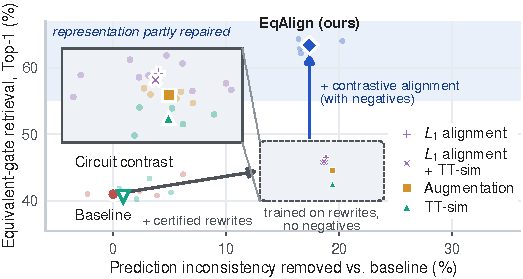
\includegraphics[width=0.9\columnwidth]{figs/fig_twolevel.pdf}}\extonly{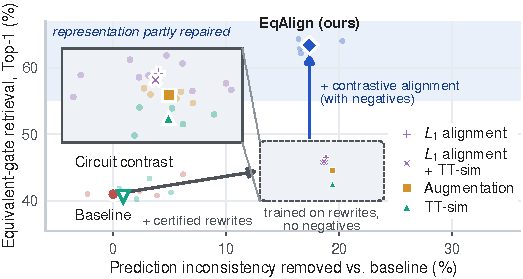
\includegraphics[width=\columnwidth]{figs/fig_twolevel.pdf}}
\caption{\textbf{Two levels of repair} on restructured pairs. \extonly{$x$: prediction inconsistency removed relative to the
baseline; $y$: Top-1 retrieval of the proven equivalent. }Small dots: seeds; large markers: 5-seed means. Inset: the
dashed box, \extonly{where every regime trained on rewrites without negatives lands (see key)}\mainonly{with every regime trained on rewrites without negatives}.}
\label{fig:twolevel}
\end{figure}


\subsection{RQ2: What Repairs It, and How Far Does the Repair Reach?}\label{sec:rq2}
\noindent\textbf{Augmentation repairs predictions, mainly under injection.} Training on certified variants lowers the
restructured inconsistency on all 7 test designs (design-level change \DTIncABDiff, 95\% CI
[\DTIncABLo,\,\DTIncABHi]) and $\rho$ under injection from \BaseRhoInj\ to \AugRhoInj, but leaves $\rho$ under synthesis
unchanged (\BaseRhoSyn\ and \AugRhoSyn), at no measurable accuracy
cost\extonly{ (MAE change \DTMaeABDiff, CI [\DTMaeABLo,\,\DTMaeABHi])}. Retrieval rises only from \BaseTopRS\% to \AugTopRS\%. Four variants per circuit instead of one add only
\EFourAugGainMin\ to \EFourAugGainMax\ points (state widths 64, 256), \EFourGapMin\ to \EFourGapMax\ below \ours\ with one\extonly{ (\cref{app:datascale})}. Representation losses without gate
correspondence fare no better (\extonly{TT-sim \TTTopRS\%, circuit-level contrast \CircTopRS\%}\mainonly{\cref{tab:main}}).


\extonly{\begin{table}[t]
\centering
\caption{\textbf{Loss weights and ablations} (seed 0); $\star$: the weight selected on validation by the rule fixed
in advance.\extonly{ The other weights of TT-sim ($\{0.5,1,2\}$) and circuit contrast (1) reach at most 33.3\% and 35.3\%
validation Top-1.}}
\label{tab:ablation}
\footnotesize\setlength{\tabcolsep}{3pt}
\resizebox{\columnwidth}{!}{\begin{tabular}{l cc cccc}
\toprule
 & \multicolumn{2}{c}{Validation} & \multicolumn{4}{c}{Test (seen families)} \\
\cmidrule(lr){2-3}\cmidrule(lr){4-7}
Variant & MAE & Top-1 & MAE & $\rho$ & Top-1 & AUROC$_\mathrm{lvl}$ \\
\midrule
Baseline & 0.0148 & 33.9 & 0.0189 & 0.97 & 41.5 & 0.766 \\
Augmentation & 0.0152 & 36.8 & 0.0177 & 0.86 & 44.8 & 0.785 \\
\midrule
\ours\ $\lambda$=0.05 & 0.0145 & 53.7 & 0.0183 & 0.80 & 61.6 & 0.856 \\
\ours\ $\lambda$=0.1 & 0.0151 & 57.0 & 0.0191 & 0.81 & 62.5 & 0.838 \\
\ours\ $\lambda$=0.2$^\star$ & 0.0166 & 58.7 & 0.0228 & 0.70 & 62.2 & 0.844 \\
\ours\ $\lambda$=0.5 & 0.0192 & 58.3 & 0.0258 & 0.72 & 60.9 & 0.858 \\
\ours\ no proj., $\lambda$=0.2 & 0.0161 & 55.9 & 0.0244 & 0.85 & 59.6 & 0.831 \\
\midrule
TT-sim $\lambda_{\mathrm{TT}}$=0.03$^\star$ & 0.0150 & 34.9 & 0.0171 & 0.94 & 40.9 & 0.768 \\
Circuit contrast $\lambda_{\mathrm{C}}$=0.2$^\star$ & 0.0167 & 39.1 & 0.0186 & 0.97 & 41.3 & 0.821 \\
\bottomrule
\end{tabular}
}
\end{table}}
\noindent\textbf{\ours\ partly repairs the representation on seen rewrites.} \ours\ raises restructured retrieval to
\OursTopRS\% (\cref{fig:twolevel}) and AUROC$_\mathrm{lvl}$ to \OursAUCHard, with the lowest $\rho$ in every column of \cref{tab:main}, partly because it errs more. The gap closed $g$
still favors it under injection (\OursGapInj\% against \BaseGapInj\% to \AugGapInj\% for the regimes of
\cref{tab:main}, on all 7 designs) but not under synthesis\extonly{ (all regimes close \BaseGapSyn\% to \OursGapSyn\%, with no
consistent difference across designs)}, where it repairs where equivalent gates sit, not what they predict.
At design level it beats the baseline by \DTTopOBDiff\ points (CI [\DTTopOBLo,\,\DTTopOBHi]) and
augmentation, TT-sim and circuit-level contrast by \DTTopOADiff, \DTTopOTDiff\ and \DTTopOCDiff\extonly{ (augmentation CI
[\DTTopOALo,\,\DTTopOAHi])}, each on all 7 designs (\extonly{each sign test $p=\DTTopOBP$; }all intervals above 0\extonly{; Welch tests over seeds against all six other regimes, Holm-adjusted: $p<\WelchHolmTopMax$}).
Simulation does better: 64-pattern signatures alone retrieve \SigRefSixtyFour\% of these pairs. \ours\ costs accuracy on original circuits: its MAE is
\OursMAECostPct\% above the baseline's (design level: \DTMaeOBDiff, CI [\DTMaeOBLo,\,\DTMaeOBHi], not significant) and
\OursMAECostAugPct\% above that of augmentation, which sees the same variants. The cost is tunable: $\lambda=0.05$
keeps baseline-level MAE at \LowLamTop\% retrieval (seed 0)\extonly{ (\cref{tab:ablation})}, and the projection head adds \NoHeadDiff\ points
(CI [\NoHeadLo,\,\NoHeadHi]).

% Fig. 4 is defined here so that it opens the right column of the page where RQ3 cites it
\begin{figure}[t]
\centering
\mainonly{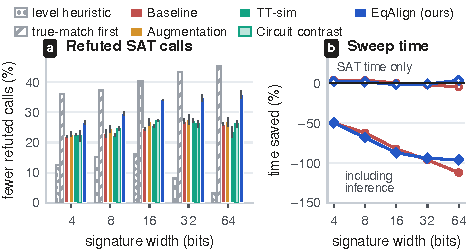
\includegraphics[width=0.92\columnwidth]{figs/fig_sweep.pdf}}\extonly{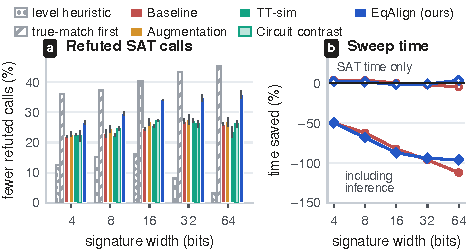
\includegraphics[width=\columnwidth]{figs/fig_sweep.pdf}}
\caption{\textbf{SAT-sweeping probe} (\extonly{5 designs $\times$ 4 variants, }pooled per seed; mean and s.e.\ over 3
seeds: GPU run in (a), CPU run in (b)). (a) Fewer refuted SAT calls than topological order; outlined: non-learned orders, filled: embeddings of
the model of that color. (b) Change in sweep time, SAT only (open) and with \extonly{embedding inference on one CPU core}\mainonly{inference} (filled).}
\label{fig:sweep}
\end{figure}
\noindent\textbf{Alignment without negatives repairs only the predictions.} \emph{$L_1$ alignment},
MixGate's loss~\cite{DBLP:journals/corr/abs-2509-20968} on our proven pairs with the weight chosen by the same rule, reaches \LoneTop\% retrieval
(\emph{$L_1$ alignment + TT-sim}: \LonettTop\%), close to augmentation's \AugTopRS\%, and the same inconsistency\extonly{;
larger weights collapse the embeddings}. Positives-only cosine alignment through the same head
retrieves \EightCosTop\%, below \ours\ on all 7 designs\extonly{ (5 seeds; \EightWDiff\ at width 256)}: here, telling
equivalent gates apart needs negatives.

\noindent\textbf{The gain needs gate correspondence and encoder training; proofs serve measurement.} Training only the projection head, with the same loss and pairs, on a frozen encoder reaches \ProbeBaseTop\% on the
baseline encoder and \ProbeAugTop\% on the augmented one: \EncShare\% of the gain over the baseline requires changing
the encoder, so it is not a readout effect\extonly{; retrieval on the encoder state instead of the projection gives
\HretTop\%}. Replacing the proven pairs by pairs matched on 4{,}096-bit or 64-bit
simulation signatures gives \SigFourKTop\% and \SigSixtyFourTop\%. The loss needs correspondences, which simulation
supplies cheaply; proofs matter for measurement.

\noindent\textbf{Repair transfers within a kind of rewrite, not across kinds, and coverage has a price.} Trained
without one synthesis script (3 seeds, widths 64 and 256; design-level means), \ours\ loses at most \TwSynCostMax\ points on it and still beats
augmentation there by \TwSynVsAugMin\ to \TwSynVsAugMax; never trained on ABC, it raises retrieval under ABC's scripts as much as
under ours (\AbcBaseTop\% to \AbcOursTop\% against \AbcBaseTopSyn\% to \AbcOursTopSyn\%), most on dc2 (\AbcBaseTopDc\% to \AbcOursTopDc\%), and in
fine-tuned DeepGate2 (\AbcFtCtrlTop\% with its own loss, \AbcFtEqTop\% with \ours); trained without injection, it retrieves \TwInjOurs\% of injected pairs
(\TwInjFull\% with them), below augmentation's \TwInjAug\% on every design\extonly{ (width 256: \TwWInjOurs\%, \TwWInjFull\% and
\TwWInjAug\%), while its retrieval under synthesis rises by \TwOthGain\ and \TwWOthGain\ points}. H2\extonly{, on which every regime
fails (\cref{tab:main}; \ours\ retrieves \OursTopHo\% on the held-out families, the baseline \BaseTopHo\%),} is
learnable: over 5 seeds, adding H2 variants to training lifts \ours's H2 retrieval from \NineEqHTwoBefore\% to
\NineEqHTwoAfter\%\extonly{ (error increase \NineEqDHTwoBefore\ to \NineEqDHTwoAfter)}, but its seen-rewrite retrieval falls from
\NineEqSeenBefore\% to \NineEqSeenAfter\% on every design and its MAE rises by \NineEqMaePct\%, at width 256 too\extonly{ (\NineEqWSeenBefore\% to \NineEqWSeenAfter\%, design-level change
\NineEqWSeenDiff\ points, CI [\NineEqWSeenLo,\,\NineEqWSeenHi]; at width 64 \NineEqSeenDiff, CI [\NineEqSeenLo,\,\NineEqSeenHi]),
and augmentation pays it too (seen retrieval \NineAugSeenBefore\% to \NineAugSeenAfter\%)}. Certified data repair the
rewrites they contain, not equivalence, and adding H2 costs invariance to the seen ones.



\subsection{RQ3: Do Aligned Embeddings Help SAT Sweeping?}\label{sec:rq3}
\noindent\textbf{The signal is real but does not pay here.} We sweep five full EPFL test designs (\extonly{ctrl, router, int2float, cavlc, adder; }174 to 1{,}020 gates) against four
certified variants each (\cref{fig:sweep})\extonly{: for every variant gate, original gates with matching $k$-bit signatures are candidates,
refined by SAT counterexamples and tried in a given order until one is proven}. Candidate orders differ only in refuted SAT
calls; the reference is topological order, as in fraiging. With 8-bit
signatures, ordering by \ours\ embeddings removes \SwOursEmbEight\% of refuted calls, against \SwBaseEmbEight\% for
baseline embeddings, \SwLevelEight\% for a logic-level heuristic and \SwTrueEight\% for trying the true match first%
\extonly{ (64-bit: \SwOursEmbSixtyFour\%, \SwBaseEmbSixtyFour\%, \SwLevelSixtyFour\%, \SwTrueSixtyFour\%)}. Here,
refuted calls on designs this small are cheap, so SAT time changes
by only \SwCpuSatTimeEight\%, while embedding inference slows the sweep at 8 bits by \SwCpuSlowEight\%
on one CPU core (\SwCpuEmbMs\,ms per circuit pair)\extonly{, and by \SwOursEmbSlowEight\% on the GPU machine, shared with training
jobs (\SwEmbMs\,ms)}. RQ3 measures equivalence information, not
DeepGate2's industrial-scale speed-up~\cite{DBLP:conf/iccad/ShiPKLLHZYCX23}.


\subsection{RQ4: Do the Findings Generalize Beyond Our Setup?}\label{sec:generality}
\newcommand{\TabGeneral}{%
\begin{table}[t]
\centering
\caption{\textbf{Generality} (seed means\extonly{; \cref{sec:generality}}). ISCAS: EPFL-trained; \extonly{$w$: state width; }\mainonly{$w$: width; }Bidir., Transf.: Top-1 over all pairs;
DG2: DeepGate2; FT: fine-tuned; $^\dagger$GPU run; --: no prob.\ head; H.-o.: \extonly{mean of H1, H2}\mainonly{held-out}\extonly{; EPFL Top-1 chance:
\DTwoChance\%}.}
\label{tab:general}
\footnotesize\setlength{\tabcolsep}{1.9pt}
\begin{tabular}{ll c ccc c cc}
\toprule
 & & MAE$\downarrow$ & \multicolumn{3}{c}{$\rho\downarrow$} & $\Delta$MAE$\downarrow$ & \multicolumn{2}{c}{Top-1 (\%)$\uparrow$} \\
\cmidrule(lr){4-6}\cmidrule(lr){7-7}\cmidrule(lr){8-9}
Setting & Model & orig. & Syn. & Inj. & H.-o. & H.-o. & seen & H.-o. \\
\midrule
\multirow{5}{*}{ISCAS} & \mk{cbase}\ Baseline & 0.0353 & 0.86 & 0.81 & 2.49 & \textbf{0.0395} & 27.0 & 14.4 \\
 & \mk{caug}\ Augmentation & \textbf{0.0332} & 0.83 & 0.56 & 2.62 & 0.0414 & 29.7 & 15.7 \\
 & \mk{ctt}\ TT-sim & 0.0333 & \textbf{0.82} & 0.55 & 2.60 & 0.0410 & 28.7 & 15.3 \\
 & \mk{ccirc}\ Circuit contrast & 0.0343 & 0.88 & 0.69 & \textbf{2.47} & 0.0409 & 29.8 & 17.3 \\
 & \hl \mk{cours}\ \ours & \hl 0.0340 & \hl \textbf{0.82} & \hl \textbf{0.50} & \hl \textbf{2.47} & \hl 0.0414 & \hl \textbf{41.8} & \hl \textbf{23.3} \\
\midrule
\multirow{3}{*}{\shortstack[l]{Bidir.\\$w{=}64$}} & \mk{cbase}\ Baseline & 0.0183 & 0.71 & 1.23 & 3.70 & 0.0509 & 49.4 & 31.9 \\
 & \mk{caug}\ Augmentation & \textbf{0.0170} & 0.70 & 0.85 & 3.88 & 0.0519 & 50.9 & 32.5 \\
 & \hl \mk{cours}\ \ours & \hl 0.0203 & \hl \textbf{0.66} & \hl \textbf{0.74} & \hl \textbf{3.35} & \hl \textbf{0.0505} & \hl \textbf{78.5} & \hl \textbf{51.4} \\
\midrule
\multirow{3}{*}{\shortstack[l]{Transf.\\$w{=}128$}} & \mk{cbase}\ Baseline & 0.0197 & 0.76 & 1.23 & \textbf{3.42} & \textbf{0.0503} & 17.5 & 12.6 \\
 & \mk{caug}\ Augmentation & \textbf{0.0184} & 0.69 & 0.81 & 3.66 & 0.0520 & 18.8 & 13.5 \\
 & \hl \mk{cours}\ \ours & \hl 0.0190 & \hl \textbf{0.68} & \hl \textbf{0.62} & \hl 3.52 & \hl 0.0517 & \hl \textbf{49.0} & \hl \textbf{31.8} \\
\midrule
\multirow{6}{*}{\shortstack[l]{Public\\(CPU)}} & DeepGate2 & 0.0287 & 0.63 & 1.01 & 2.54 & 0.0468 & 37.4 & 22.6 \\
 & DG2 retrained$^\dagger$ & 0.0479 & 0.51 & 0.75 & 1.69 & 0.0446 & 35.3 & 22.3 \\
 & DG3 tokenizer & 0.0214 & 0.85 & 1.34 & 3.82 & 0.0510 & 42.9 & 28.5 \\
 & FGNN2 & -- & -- & -- & -- & -- & 61.9 & 43.5 \\
 & MGVGA & -- & -- & -- & -- & -- & 20.4 & 12.7 \\
 & TRACE & -- & -- & -- & -- & -- & 66.6 & 43.6 \\
\midrule
\multirow{2}{*}{\shortstack[l]{FT\\(GPU)}} & DG2 + own loss & \textbf{0.0269} & \textbf{0.66} & 0.78 & 2.80 & 0.0501 & 40.1 & 23.6 \\
 & \hl \mk{cours}\ DG2 + \ours & \hl 0.0322 & \hl 0.68 & \hl \textbf{0.63} & \hl \textbf{2.29} & \hl \textbf{0.0465} & \hl \textbf{66.6} & \hl \textbf{39.2} \\
\bottomrule
\end{tabular}

\end{table}}
\mainonly{\TabGeneral}
\noindent\textbf{Confirmatory design.} With all other results fixed, we evaluated the 15 CPU-run models
(5 regimes, 3 seeds) on \HypCones\ hyp circuits\extonly{; the 25 GPU models,
evaluated later, agree (\ours\ \HypGpuOursTop\% against at most \HypGpuBestOtherTop\%, its worst seed \HypGpuOursTopMin\% above every other
regime's best, \HypGpuOtherTopMax\%)}. The main findings replicate: the baseline's $\rho$ under
synthesis is \HypBaseRhoSyn, augmentation lowers $\rho$ under injection (\HypBaseRhoInj\ to \HypAugRhoInj), H2 raises every
regime's matched-gate error by \HypHTwoMin\ to \HypHTwoMax, and \ours\ retrieves \HypOursTop\% against at most
\HypBestOtherTop\% otherwise\extonly{ (worst \ours\ seed \HypOursTopMin\%, best
other \HypOtherTopMax\%). Two secondary findings do not: \ours's AUROC$_\mathrm{lvl}$ (\HypOursAUC) does not exceed the other
representation losses' (up to \HypBestOtherAUC), and it pays no accuracy cost there (MAE \HypOursMAE, the lowest)}.

\extonly{\TabGeneral}
\noindent\textbf{Second benchmark suite.} On ISCAS85/89, with EPFL-trained models, synthesis moves
baseline predictions\extonly{ by $\rho=\ISBaseRhoSyn$}, H2 breaks every regime, and \ours\ raises retrieval\extonly{ from
\ISBaseTopRS\% to \ISOursTopRS\%}, beyond every other regime\extonly{ tested} on all \IsDesN\ designs (\extonly{design-level gaps \IsDesTopMin\ to \IsDesTopMax\ points, }Holm-adjusted
sign test $p<10^{-4}$; \cref{tab:general}).

\noindent\textbf{ABC synthesis scripts.} Under ABC's scripts, all \AbcNArch\ baseline encoders (3 architectures, 3 widths each) stay blind ($\rho$ \AbcAllRhoMin\ to \AbcAllRhoMax, against
\AbcAllRhoSynMin\ to \AbcAllRhoSynMax\ under ours; released DeepGate2: \AbcDTwoRho) with no rise in matched-gate error; augmentation does
not lower the inconsistency (all intervals include 0), and the recurrent \ours\ beats every regime on all 7 designs at width 64
and on all but ctrl (16 cones) at width 256 (gains: \cref{sec:rq2})\extonly{; on ISCAS it raises retrieval from \AbcIsBaseTop\% to \AbcIsOursTop\%, and in fine-tuned DeepGate2 from
\AbcIsFtCtrlTop\% to \AbcIsFtEqTop\% (\cref{app:abc})}.

\noindent\textbf{Other architectures.} A bidirectional encoder (attention, reverse pass)
and a transformer show the two levels at every width tested (64 to 512): \ours\ raises retrieval\extonly{ over all
proven pairs from \BiBaseTopRS\% to \BiOursTopRS\% and from \TfBaseTopRS\% to \TfOursTopRS\%}\mainonly{ (\cref{tab:general})}, beyond every other regime\extonly{ tested} on all 7
designs, and all fail on H2\extonly{; augmentation lowers $\rho$ under injection from \BiBaseRhoInj\ to \BiAugRhoInj\ and
from \TfBaseRhoInj\ to \TfAugRhoInj\ (all widths: \cref{tab:app_arch})}.

\noindent\textbf{Released checkpoints.} We ran \audit\ unchanged on the functional embedding $\mathbf h_f$ of released
DeepGate2 and the DeepGate3 tokenizer (released without its refining transformer); both were trained on
subcircuits that include EPFL designs~\cite{DBLP:conf/iccad/ShiPKLLHZYCX23,DBLP:conf/iccad/ShiZKZ0024}. \extonly{Both draw fresh random primary-input vectors per
forward pass, so the same circuit retrieves only \DTwoSelfRand\% and \DThreeSelfRand\% of its own gates; we share
them across a rewrite, which changes no conclusion. }Both show the pattern (\cref{tab:general}): \extonly{re-synthesis moves the prediction
for a fixed function by \DTwoRhoSyn\ and \DThreeRhoSyn\ times the model's error, and the held-out families take
retrieval from \DTwoTopSeen\% and \DThreeTopSeen\% to \DTwoTopHo\% and \DThreeTopHo\%}\mainonly{predictions move under re-synthesis and retrieval falls under held-out families} (H2 alone: \DTwoHTwoRS\% and \DThreeHTwoRS\%). Retrained with its released code and data
(\TenSeeds\ seeds), DeepGate2 errs more than its released weights\extonly{ (MAE \TenMAE\ vs.\ \TenRelMAE)} yet disagrees nearly as much (\TenIncons\ vs.\ \TenRelIncons) and fails alike (\extonly{\TenTop\% seen, }\TenHTwo\% under H2): blindness
is not specific to one checkpoint, and higher accuracy did not reduce it\extonly{ (its lower
$\rho$ in \cref{tab:general} reflects the larger error in the denominator, not a smaller disagreement)}.\extonly{ From DeepGate2 to DeepGate3's tokenizer, the restructured error falls by
\DThreeErrDrop\% but the disagreement across a rewrite by only \DThreeInconsDrop\%.}

\noindent\textbf{Released gate-state encoders.} TRACE, MGVGA and FGNN2~\cite{DBLP:conf/dac/ZhengZZX26,DBLP:conf/iclr/WuZ0025,DBLP:journals/tcad/WangBHZXHHY25} have no
probability head; we audit their gate states\extonly{, with input conventions fixed by each model's own pretraining
objective (\cref{app:ext})}. TRACE and FGNN2, trained for equivalence, retrieve
\extonly{\TrSeen\% and \FgSeen\% on seen rewrites, the most of any released encoder,}\mainonly{the most of any released encoder on seen rewrites (\cref{tab:general})} but \TrHTwo\% and \FgHTwo\% under H2;
MGVGA, which gives many gates identical embeddings (\MgSelf\% retrieval within an identical copy), gets \extonly{\MgSeen\% and \MgHTwo\% (H2)}\mainonly{\MgHTwo\% under H2}.

\noindent\textbf{Repairing a released model.} Fine-tuning released DeepGate2 on our training data
(5 epochs, \FtEqSeeds\ seeds) with its own loss moves retrieval from \TenRelTop\% (released weights, GPU evaluation) to \FtCtrlTopSeen\%; adding \ours\ on $\mathbf h_f$
reaches \FtEqTopSeen\% (higher on all 7 designs\extonly{, design-level gain \FtDiff\ points}\extonly{, CI [\FtDiffLo,\,\FtDiffHi]}; held-out \FtEqTopHo\% vs.\
\FtCtrlTopHo\%) at \FtMaeCostPct\% higher MAE.

\noindent\textbf{Model and circuit size.} Growing the encoder \ScFold-fold (recurrent widths 64 to 1024, \ScMinParams\ to
\ScMaxParams\ parameters, and 4 instead of 2 passes; transformers 128 to 512) leaves blindness intact: the recurrent baseline's $\rho$ under synthesis
stays between \ScBaseRhoMin\ and \ScBaseRhoMax\ and its retrieval drifts from \ScBaseTopFirst\% to \ScBaseTopLast\%, while \ours\ leads the
baseline and augmentation by \ScLeadMin\ to \ScLeadMax\ design-level points at every size, on all 7 designs\extonly{ (5 seeds each; at width
256 it leads every regime by \WDiffMin\ to \WDiffMax\ points, and synthesis inconsistency is \WNoise\ times the seed noise floor;
all sizes: \cref{tab:app_scale})}. On \LgCones\ test circuits of \LgGatesMin\ to \LgGatesMax\ gates (median \LgGatesMed) from \LgDesigns\ arithmetic
designs, retrieval falls for every regime as candidates multiply (chance \LgChance\%): the baseline retrieves
\LgBaseTop\%, \ours\ \LgOursTop\%, above every other regime (at most \LgOtherMax\%) on all \LgDesigns\ designs (Welch $p<10^{-4}$\extonly{, Holm-adjusted; too few designs for a design-level test}); none exceeds \LgHTwoMax\% under H2\extonly{; width 256 gives \LgWBaseTop\%, \LgWOursTop\% and at most \LgWOtherMax\%}.